\newpage\section{Fehlerfortpflanzung}
\subsection{a)}
Ohne Korrelation:
\begin{align}
\sigma_y &= \sqrt{\biggl( \frac{\partial y}{\partial a_0}\cdot \sigma_{a_0}\biggr)^2 
+\biggl( \frac{\partial y}{\partial a_1}\cdot \sigma_{a_1}\biggr)^2}\\
&= \sqrt{( \sigma_{a_0})^2 
+ ( x^2\cdot \sigma_{a_1})^2}\\
&= \sqrt{\SI{0.04}{} + x^2 \cdot \SI{0.04}{}}\\
&= \SI{0.2}{}\sqrt{1+x^2}
\end{align}
Mit Korrelation:
\begin{align}
\sigma_y &= \sqrt{\biggl( \frac{\partial y}{\partial a_0}\cdot \sigma_{a_0}\biggr)^2 
+\biggl( \frac{\partial y}{\partial a_1}\cdot \sigma_{a_1}\biggr)^2
+2\cdot\biggl(\frac{\partial y}{\partial a_0}\biggr)\biggl(\frac{\partial y}{\partial a_1}\biggr)\cdot \text{cov}(a_0,a_1)}\\
&= \sqrt{( \sigma_{a_0})^2 
+ ( x^2\cdot \sigma_{a_1})^2
+ 2x \rho\sigma_{a_0}\sigma_{a_1}}\\
&= \sqrt{\SI{0.04}{} + x^2 \cdot \SI{0.04}{} + 2x\cdot(\SI{-0.032}{})}\\
&= \SI{0.2}{}\sqrt{1+x(x-\SI{1.6}{})}
\end{align}
\subsection{b)}
\begin{center}
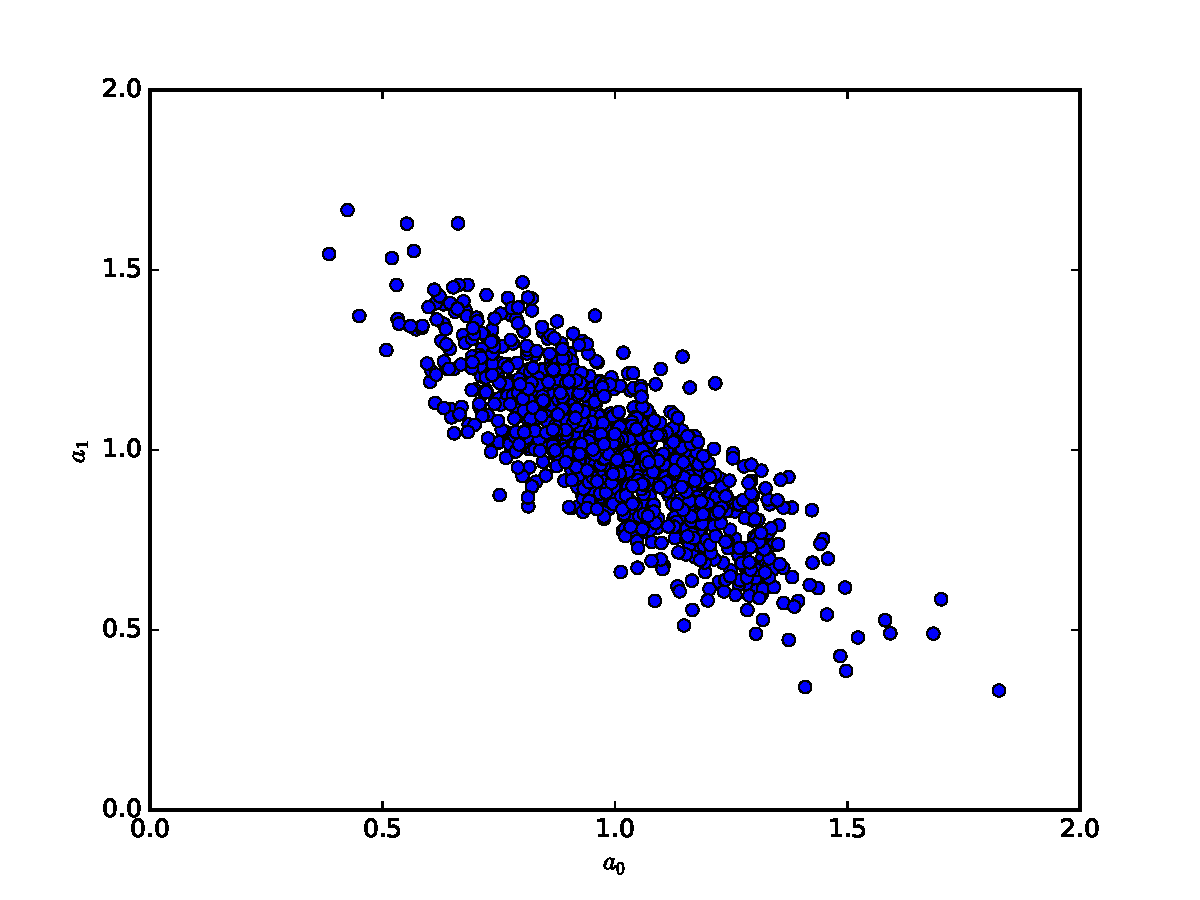
\includegraphics[width=0.7\linewidth]{A4_abgabe.pdf}
\end{center}
Die beiden normalverteilten Zufallsverteilungen enthalten jeweils $n=1000$ Einträge. Ihre Standardabweichungen sind $\sigma_{a_0}=\SI{0.196553916}{}$ und $\sigma_{a_0}=\SI{0.201931815}{}$. Die zu den Verteilungen gehörenden Mittelwerte habe ich leider nicht mit aufgezeichnet. Da ich nicht noch die Zahlenwerte bei c) an andere Verteilungen anpassen möchte, fehlen sie hier, auch wenn sie interessant wären.

\subsection{c)}
Analytisch:
\begin{align}
\mu_y &= \mu_{a_0} + x\cdot \mu_{a_1}\\
& = \SI{1}{}+ x\\
\sigma_y &= \SI{0.2}{}\sqrt{1+x(x-\SI{1.6}{})}\\ \\
y(\SI{-3}{})&=\SI{-2.000000000(769415362)}{}&=\SI{-2.0(8)}{}\\
y(\SI{0}{})&=\SI{1.0(2)}{}\\
y(\SI{3}{})&=\SI{4.000000000(456070170)}{}&=\SI{4.0(5)}{}
\end{align}
Numerisch:
\begin{align}
y(x) &= {a_0} + x\cdot {a_1}\\
y(\SI{-3}{})&=\SI{-1.993234617(774074662)}{}&=\SI{-2.0(8)}{}\\
y(\SI{0}{})&=\SI{1.000371543(196553916)}{}&=\SI{1.0(2)}{}\\
y(\SI{3}{})&=\SI{3.993977704(460490551)}{}&=\SI{4.0(5)}{}
\end{align}
Es ist zu erkennen, dass die numerisch simulierten Werte mit den analytisch berechneten Werten (auf signifikante Stellen gerundet exakt) Übereinstimmen. Es ist weder bei den der Mittelwerte, noch bei den Standardabweichungen ein Muster in den Abweichungen zwischen analytisch und numerisch bestimmten Werten ersichtlich.
\newline (Auch bei Wiederholungen mit anderen Zufallsverteilungen ändert sich dies nicht. Je größer die Zahl $n$ der Einträge wird, desto genauer stimmen die numerischen Erte mit den analytisch berechneten überein, da auch die Verteilungen $a_0$ und $a_1$ den Vorgaben genauer entsprechen.)
